\section{检验三段论:文恩图解法}

\begin{quotation}
文恩图是检验三段论有效性的直观而强大的工具。本节介绍如何使用三圆文恩图同时表示三段论的两个前提,并根据图示判断论证是否有效。这种方法不仅能够检验特定论证的有效性,还能证明某种形式的所有三段论都是有效的或无效的。
\end{quotation}

前一章已经介绍了两个圆的文恩图如何用于描述标准式三段论的命题。要运用文恩图解法检验直言三段论,就必须把两个前提在同一个图示中描述出来。这就要求画相互重叠的三个圆,因为标准式三段论有两个前提,共包含着三个不同的项——大项、小项和中项——分别记为 $S$、$P$ 和 $M$。我们首先并列画两个交叉圆,与图示单个命题一样,然后再在其下方画出第三个圆,与前两个圆都有重叠部分,依次给三个圆标记 $S$、$P$ 和 $M$。既然一个圆既能表示类 $S$ 也能表示类 $\bar{S}$,标有 $S$ 和 $P$ 的两个交叉的圆能表示四个类,即 $SP$、$S\bar{P}$、$\bar{S}P$ 和 $\overline{SP}$。这样,标有 $S$、$M$ 和 $P$ 的三个交叉的圆可以表示八个类:$S\overline{PM}$、$SP\bar{M}$、$\bar{S}P\bar{M}$、$S\bar{P}M$、$SPM$、$\bar{S}PM$、$\overline{SP}M$ 和 $\overline{SPM}$。三个圆可以将其所在平面分为八个部分,它们分别表示了上列八个类,见图 6-1。

\begin{center}
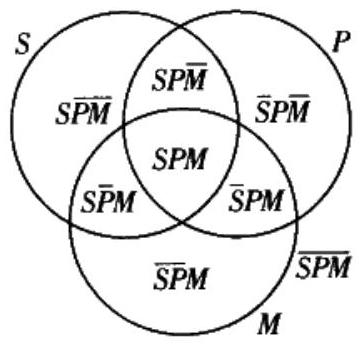
\includegraphics[width=\textwidth]{images/2025_05_15_6a28331d5e7c993ad07ag-274.jpg}

图6-1 三圆文恩图的八个区域
\end{center}

以瑞典人的类($S$)、农民的类($P$)和音乐家的类 ($M$) 为例,可以作如下解释。$SPM$ 是这三个类的积,由所有瑞典农民音乐家组成。$SP\bar{M}$是前两个类与第三个类之补的积,由不是音乐家的瑞典农民组成。$S\bar{P}M$是第一、第三个类与第二个类之补的积:所有不是农民的瑞典音乐家组成的类。$S\overline{PM}$ 是第一个类与其他两个类之补的积:所有不是农民也不是音乐家的瑞典人组成的类。接下来,$\bar{S}PM$ 是第二、第三个类与第一个类之补的积:所有不是瑞典人的农民音乐家组成的类。$\bar{S}P\bar{M}$ 是第二个类与其他两个类之补的积:所有不是瑞典人也不是音乐家的农民组成的类。$\overline{SP}M$ 是第三个类与前两个类之补的积:所有不是瑞典人也不是农民的音乐家组成的类。最后,$\overline{SPM}$ 是三个类的补的积:所有不是瑞典人、不是农民,也不是音乐家的事物组成的类。

我们把注意力集中到标有 $P$ 和 $M$ 的两个圆上,显然,加上阴影或写入 $x$ 就能表示出 $P$、$M$ 构成的任何标准式直言命题,无论哪个是主项哪个是谓项。例如,要用图表示命题"所有 $M$ 是 $P$"($M\bar{P}=0$),我们就把所有不包含在 $P$ 中的 $M$ 的部分加上阴影。这个区域,包括了标有 $S\bar{P}M$ 和 $\overline{SP}M$ 的部分,这样就形成了图6-2。

\begin{center}
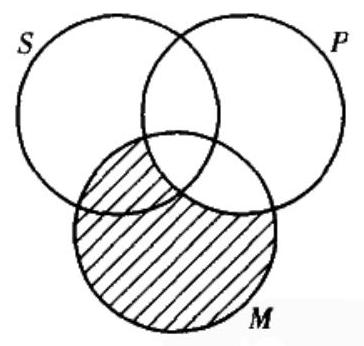
\includegraphics[width=\textwidth]{images/2025_05_15_6a28331d5e7c993ad07ag-275(2).jpg}

图6-2 "所有$M$是$P$"的表示
\end{center}

我们再把注意力集中到 $S$ 和 $M$,加上阴影或写入 $x$ 就能表示由 $S$、$M$ 构成的任何标准式直言命题,无论它们出现的顺序。要用图表示命题"所有 $S$ 是 $M$"($S\bar{M}=0$),我们就把所有不包含在 $M$ 中的 $S$ 的部分加上阴影。这个区域,包括了标有 $S\overline{PM}$ 和 $SP\bar{M}$ 的部分。这样就形成了图 6-3。

\begin{center}
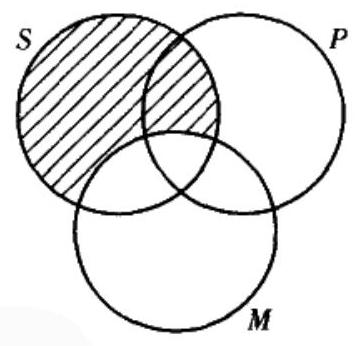
\includegraphics[width=\textwidth]{images/2025_05_15_6a28331d5e7c993ad07ag-275(1).jpg}

图6-3 "所有$S$是$M$"的表示
\end{center}

现在,利用三个交叉的圆,就可以在一个图中同时表示两个命题——当然,条件是其中只出现三个不同的项。这样,"所有 $M$ 是 $P$"和"所有 $S$ 是 $M$"可以同时表示在图6-4中。

\begin{center}
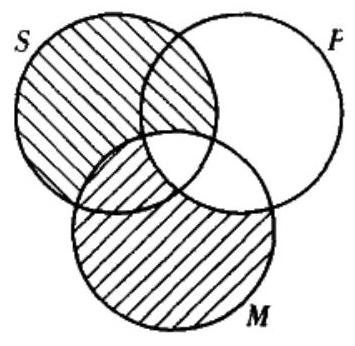
\includegraphics[width=\textwidth]{images/2025_05_15_6a28331d5e7c993ad07ag-275.jpg}

图6—4 两个前提"所有$M$是$P$"和"所有$S$是$M$"的表示
\end{center}

这正是三段论 AAA-1 的两个前提:
\begin{quote}
所有$M$是$P$\\
所有$S$是$M$\\
所以,所有$S$是$P$
\end{quote}

此三段论是有效的,当且仅当两个前提蕴涵或曰能推出结论,即两个前提已断言了结论所断言的东西。因此,在文恩图中画出有效论证的前提,也就已经把结论画出来了,而不需要画更多的圆。结论"所有 $S$ 是 $P$"的文恩图,应为在标有 $S\overline{P\bar{M}}$ 和 $S\bar{P}M$ 的部分加上阴影。我们看到表示两个前提的文恩图,也确实已经把结论表示了出来。这种情况说明 AAA-1 一定是有效式。$^{[3]}$

我们再用文恩图检验一个明显无效的三段论:

\begin{quote}
所有狗是动物,\\
所有猫是动物,\\
所以,所有猫是狗。
\end{quote}

用文恩图表示两个前提就是图6-5。

\begin{center}
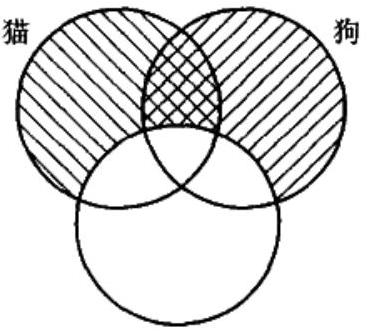
\includegraphics[width=\textwidth]{images/2025_05_15_6a28331d5e7c993ad07ag-276.jpg}

图6-5 "所有狗是动物,所有猫是动物"的表示
\end{center}

在这个图中,$S$ 指称所有猫组成的类,$P$ 指称所有狗组成的类,而 $M$指称所有动物组成的类,$S\overline{PM}$、$SP\bar{M}$ 和 $\bar{S}P\bar{M}$ 部分已经加上了阴影,但结论却没有被表示出来,因为 $S\bar{P}M$ 部分没有阴影,要图示结论就必须把 $S\overline{PM}$ 和 $S\bar{P}M$ 两部分都加上阴影。这样,就能看出 AAA-2 的两个前提的图示并没能表示结论,这证明结论的断定超出了前提,前提并不蕴涵结论。而一个前提不蕴涵结论的论证是无效的,所以,我们所画出的图示证明了这个三段论是无效的。(实际上,它证明任何形如 AAA-2 的三段论都是无效的。)

如果我们用文恩图检验由一个全称前提和一个特称前提构成的三段论,那么,很重要的一点是:要首先在图中表明全称前提。举例来说,要检验下面的三段论:

\begin{quote}
所有艺术家都是自我主义者,\\
有艺术家是乞丐,\\
所以,有乞丐是自我主义者。
\end{quote}

我们应当先画出全称前提"所有艺术家都是自我主义者",再写入 $x$ 表示特称前提"有艺术家是乞丐"。正确的图示见图 6-6。

\begin{center}
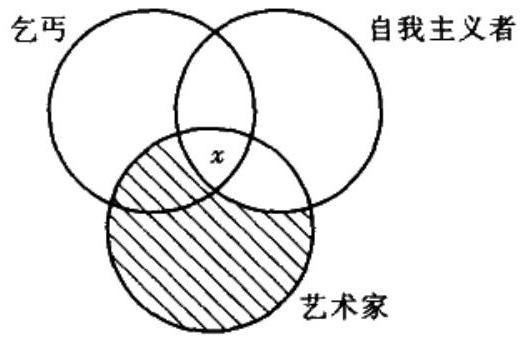
\includegraphics[width=\textwidth]{images/2025_05_15_6a28331d5e7c993ad07ag-277.jpg}

图6-6 "所有艺术家都是自我主义者,有艺术家是乞丐"的表示
\end{center}

$S\bar{P}M$ 连同 $\overline{SP}M$ 两个部分表明的是全称前提,如果在给这两个部分加上阴影之前,试图先表明特称前提,我们就不能确定到底该把 $x$ 加在 $SPM$ 部分还是 $S\bar{P}M$ 部分,或者两个部分都加上。如果加在 $S\bar{P}M$ 当中,或者加在这部分与 $SPM$ 的交界处,那么加在 $S\bar{P}M$ 中的阴影就让图的原意变得含混不清。既然前提中包含的信息已经表示在图中了,检验时就看它是否也表明了结论。如果结论"有乞丐是自我主义者"能被表示出来,就应该把 $x$ 放在"乞丐"和"自我主义者"两个类的交叉部分。这个部分既包含了 $SPM$ 也包含 $\bar{S}PM$ 部分,它们共同表明 $SP$。此三段论的结论所断定的东西,已经在表示前提的图示中表明了,因此,这个三段论是有效的。

再来看另一个例子,对这个例子的讨论将说明文恩图一个更重要的作用。考虑论证:

\begin{quote}
所有大科学家都是大学毕业生,\\
有职业运动员是大学毕业生,\\
所以,有职业运动员是大科学家。
\end{quote}

首先在 $SP\bar{M}$ 和 $\bar{S}P\bar{M}$ 部分加上阴影,这样就表明了全称前提(见图6— 7),但我们仍然不明白应该把 $x$ 加到哪一部分才能表明特称前提。特称前提是"有职业运动员是大学毕业生",所以 $x$ 必须加在标有"职业运动员"和"大学毕业生"的两个圆交叉的部分。但是,交叉的区域又包括两个部分:$SPM$ 和 $S\bar{P}M$。$x$ 应该放到其中哪个部分呢?前提并没有告诉我们答案,如果任意选一部分把 $x$ 加上去,就可能在图中加上了一些前提中本来没有的信息——也就破坏了文恩图检验的有效性。如果在两个部分都加一个 $x$,也会超出前提的断言。但是,把 $x$ 放在两部分的交界线上,我们就正好表明了第二个前提,而没有提供任何更多的东西。$x$ 放在交界线上,指的是有东西属于它们两个类中的一个,但确实没有说明到底属于哪一类。两个前提的完整图示见图 6-8。

\begin{center}
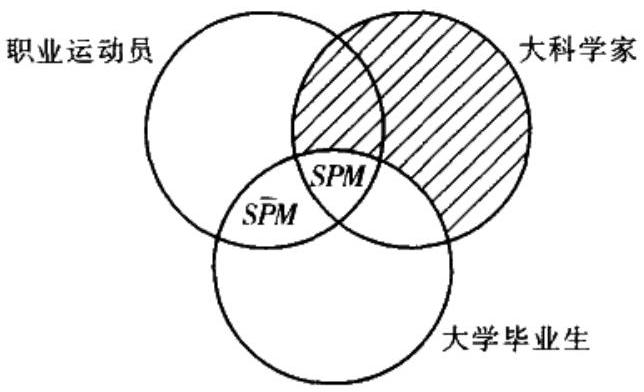
\includegraphics[width=\textwidth]{images/2025_05_15_6a28331d5e7c993ad07ag-278.jpg}

图 6-7 "所有大科学家都是大学毕业生"的表示
\end{center}

\begin{center}
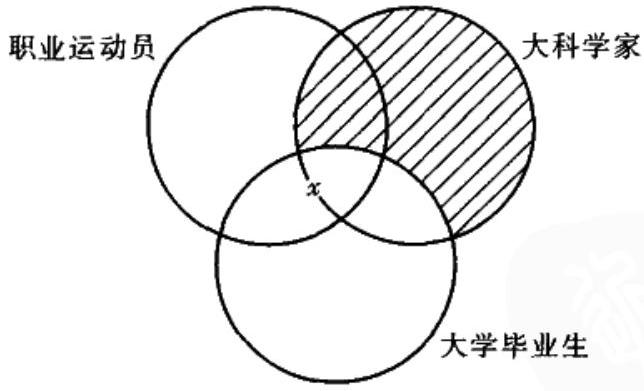
\includegraphics[width=\textwidth]{images/2025_05_15_6a28331d5e7c993ad07ag-278(1).jpg}

图6-8 "所有大科学家都是大学毕业生,有职业运动员是大学毕业生"的表示
\end{center}

通过考察,我们会发现前提的图示中并没有把结论表达出来。要表明结论"有职业运动员是大科学家",就必须要加一个 $x$ 在上面两个圆的交叉部分,或者加在 $SP\bar{M}$ 中,或者加在 $SPM$ 中。前面一个部分已经被加上阴影排除出去了,当然就不会包含 $x$。但图示也并没有显示 $SPM$ 中有 $x$。确实,$SPM$ 或者 $S\bar{P}M$ 之中必有一个元素,但这个图示并没有说明究竟是在前者当中,还是在后者当中,因为前提就没有说明这一点。所以,结论就可能为假。当然,我们由此并不能确定结论就是假的,而只能知道结论没有被前提断定或蕴涵。但这已足以告诉我们论证是无效的。这个图也充分说明并非只有给定的这个三段论是无效的,而是所有形如 AII-2 的三段论都是无效的。

使用文恩图检验标准式三段论的一般做法可以总结如下:首先,在三圆的文恩图上标记三段论的三个项。接下来,把两个前提在图中都表示出来,如果一个前提是全称、另一个是特称的话,要首先标明全称前提。特别注意,如果特称前提并没有明确表明应该把 $x$ 加在哪一部分时,就把 $x$放在两个部分的交叉线上。最后,检查图示中是否已经包含了结论:如果包含了,那么三段论就是有效的,否则就是无效的。

使用文恩图区分三段论有效性与无效性的理论依据是什么?这个问题的答案可分为两个部分。首先,必须结合 6.2 节讲到的三段论论证的形式性质来讨论。那一节讲过,对给定三段论有效还是无效的一种合理检验是去判定另外一个三段论的有效性如何,而这个三段论与要考察的三段论恰有相同的形式。这种方法正是文恩图解法的基本依据。而说明文恩图解法如何达到这种检验目标,就构成问题解答的第二部分。

三段论一般都是就对象类而言的,其中的对象并不都呈现在我们面前,比如音乐家的类、大科学家的类、钠盐的类等等。这些类之间的包含或排斥关系可能是由论证得出的,也可能是在科学研究过程中经验地发现的。但它们绝不会自己呈现出来,因为涉及的类的元素不可能全部展现出来接受观察。但我们可创设一种情形,在这种经特殊界定的情形中,所涉及各个类的元素都可以呈现在人们面前以供直接观察,从而可以构造关于这种自设情形的三段论论证。文恩图本来是为表示标准直言命题而发明的,但其亦属于一种创设情形,一种可以使用各种工具在纸上、在黑板上绘制出来的情形。其所表示的命题亦可以解释为指涉图形本身。兹举一例即可说明。假如我们有这样一个关于分布在世界各地的各色人等的特殊三段论,其词项分别指称成功人士、热爱工作者和心猿意马者(工作中注意力分散者):

\begin{quote}
所有成功人士都是热爱工作者,\\
没有热爱工作者是心猿意马者,\\
所以,没有心猿意马者是成功人士。
\end{quote}

它的形式是 AEE-4,即:

\begin{quote}
所有 $P$ 是 $M$,\\
没有 $M$ 是 $S$,\\
$\therefore$ 没有 $S$ 是 $P$。
\end{quote}

\footnotetext{(3)在使用文恩图中,我们同样也采用5.6节提到的布尔解释。因此,对当方阵中只有矛盾关系成立,而下反对、反对和上下位差等关系不存在。}

\begin{center}
\fbox{\parbox{0.95\textwidth}{
\textbf{本节要点}
\begin{itemize}
\item \textbf{文恩图解法}:使用三个重叠的圆表示三个词项,并在同一图中表示两个前提
\item 文恩图中的\textbf{三圆八区域}对应于三类项及其补类的各种组合
\item 使用文恩图检验三段论的步骤:
  \begin{itemize}
  \item 标记三个词项(大项$P$、小项$S$和中项$M$)
  \item 在图中表示两个前提(全称前提用阴影,特称前提用$x$)
  \item 若图中已包含结论,则三段论有效;否则无效
  \end{itemize}
\item 特称前提与全称前提同时表示时的注意事项:
  \begin{itemize}
  \item 先表示全称前提
  \item 特称前提的$x$若位置不确定,应放在区域交界线上
  \end{itemize}
\item 文恩图不仅可以检验单个论证,还能证明整个形式的有效性或无效性
\end{itemize}
}}
\end{center} 